%% BioMed_Central_Tex_Template_v1.05
%%                                      %
%  bmc_article.tex            ver: 1.05 %
%                                       %


%%%%%%%%%%%%%%%%%%%%%%%%%%%%%%%%%%%%%%%%%
%%                                     %%
%%  LaTeX template for BioMed Central  %%
%%     journal article submissions     %%
%%                                     %%
%%         <27 January 2006>           %%
%%                                     %%
%%                                     %%
%% Uses:                               %%
%% cite.sty, url.sty, bmc_article.cls  %%
%% ifthen.sty. multicol.sty		       %%
%%									   %%
%%                                     %%
%%%%%%%%%%%%%%%%%%%%%%%%%%%%%%%%%%%%%%%%%


%%%%%%%%%%%%%%%%%%%%%%%%%%%%%%%%%%%%%%%%%%%%%%%%%%%%%%%%%%%%%%%%%%%%%
%%                                                                 %%	
%% For instructions on how to fill out this Tex template           %%
%% document please refer to Readme.pdf and the instructions for    %%
%% authors page on the biomed central website                      %%
%% http://www.biomedcentral.com/info/authors/                      %%
%%                                                                 %%
%% Please do not use \input{...} to include other tex files.       %%
%% Submit your LaTeX manuscript as one .tex document.              %%
%%                                                                 %%
%% All additional figures and files should be attached             %%
%% separately and not embedded in the \TeX\ document itself.       %%
%%                                                                 %%
%% BioMed Central currently use the MikTex distribution of         %%
%% TeX for Windows) of TeX and LaTeX.  This is available from      %%
%% http://www.miktex.org                                           %%
%%                                                                 %%
%%%%%%%%%%%%%%%%%%%%%%%%%%%%%%%%%%%%%%%%%%%%%%%%%%%%%%%%%%%%%%%%%%%%%


\NeedsTeXFormat{LaTeX2e}[1995/12/01]
\documentclass[10pt]{bmc_article}    



% Load packages
\usepackage{cite} % Make references as [1-4], not [1,2,3,4]
\usepackage{url}  % Formatting web addresses  
\usepackage{ifthen}  % Conditional 
\usepackage{multicol}   %Columns
\usepackage[utf8]{inputenc} %unicode support
%\usepackage[applemac]{inputenc} %applemac support if unicode package fails
%\usepackage[latin1]{inputenc} %UNIX support if unicode package fails
\urlstyle{rm}
\usepackage{graphicx}
\usepackage{color}

\usepackage[dvips]{epsfig}
\usepackage[]{ulem}
\usepackage[]{algorithmic}
\usepackage{epstopdf}
\usepackage[lofdepth,lotdepth]{subfig}
 
\newtheorem{mydef}{Definition}
 
%%%%%%%%%%%%%%%%%%%%%%%%%%%%%%%%%%%%%%%%%%%%%%%%%	
%%                                             %%
%%  If you wish to display your graphics for   %%
%%  your own use using includegraphic or       %%
%%  includegraphics, then comment out the      %%
%%  following two lines of code.               %%   
%%  NB: These line *must* be included when     %%
%%  submitting to BMC.                         %% 
%%  All figure files must be submitted as      %%
%%  separate graphics through the BMC          %%
%%  submission process, not included in the    %% 
%%  submitted article.                         %% 
%%                                             %%
%%%%%%%%%%%%%%%%%%%%%%%%%%%%%%%%%%%%%%%%%%%%%%%%%                     


%\def\includegraphic{}
%\def\includegraphics{}



\setlength{\topmargin}{0.0cm}
\setlength{\textheight}{21.5cm}
\setlength{\oddsidemargin}{0cm} 
\setlength{\textwidth}{16.5cm}
\setlength{\columnsep}{0.6cm}

\newboolean{publ}

%%%%%%%%%%%%%%%%%%%%%%%%%%%%%%%%%%%%%%%%%%%%%%%%%%
%%                                              %%
%% You may change the following style settings  %%
%% Should you wish to format your article       %%
%% in a publication style for printing out and  %%
%% sharing with colleagues, but ensure that     %%
%% before submitting to BMC that the style is   %%
%% returned to the Review style setting.        %%
%%                                              %%
%%%%%%%%%%%%%%%%%%%%%%%%%%%%%%%%%%%%%%%%%%%%%%%%%%
 

%Review style settings
\newenvironment{bmcformat}{\begin{raggedright}\baselineskip20pt\sloppy\setboolean{publ}{false}}{\end{raggedright}\baselineskip20pt\sloppy}

%Publication style settings
%\newenvironment{bmcformat}{\fussy\setboolean{publ}{true}}{\fussy}



% Begin ...
\begin{document}
\begin{bmcformat}


%%%%%%%%%%%%%%%%%%%%%%%%%%%%%%%%%%%%%%%%%%%%%%
%%                                          %%
%% Enter the title of your article here     %%
%%                                          %%
%%%%%%%%%%%%%%%%%%%%%%%%%%%%%%%%%%%%%%%%%%%%%%

\title{Towards speed up of Whole Genome Alignment using Distributed Suffix Tree}
 
%%%%%%%%%%%%%%%%%%%%%%%%%%%%%%%%%%%%%%%%%%%%%%
%%                                          %%
%% Enter the authors here                   %%
%%                                          %%
%% Ensure \and is entered between all but   %%
%% the last two authors. This will be       %%
%% replaced by a comma in the final article %%
%%                                          %%
%% Ensure there are no trailing spaces at   %% 
%% the ends of the lines                    %%     	
%%                                          %%
%%%%%%%%%%%%%%%%%%%%%%%%%%%%%%%%%%%%%%%%%%%%%%


\author{Julio Cesar Garcia Vizcaino\correspondingauthor$^{1}$%
       \email{Julio Cesar Garcia Vizcaino\correspondingauthor - juliocesar.garcia@e-campus.uab.cat}%
      \and
       and 
         Antonio Espinosa$^2$%
         \email{Antonio Espinosa - antonio.espinosa@caos.uab.es}%
      }
      

%%%%%%%%%%%%%%%%%%%%%%%%%%%%%%%%%%%%%%%%%%%%%%
%%                                          %%
%% Enter the authors' addresses here        %%
%%                                          %%
%%%%%%%%%%%%%%%%%%%%%%%%%%%%%%%%%%%%%%%%%%%%%%

\address{%
    \iid(1)Computer Architecture \& Operating Systems Department (CAOS), Universitat Autònoma de Barcelona,%
    Bellaterra (Barcelona), Spain.\\
    \iid(2)Computer Architecture \& Operating Systems Department (CAOS), Universitat Autònoma de Barcelona,%
    Bellaterra (Barcelona), Spain.
}%

\maketitle

%%%%%%%%%%%%%%%%%%%%%%%%%%%%%%%%%%%%%%%%%%%%%%
%%                                          %%
%% The Abstract begins here                 %%
%%                                          %%
%% The Section headings here are those for  %%
%% a Research article submitted to a        %%
%% BMC-Series journal.                      %%  
%%                                          %%
%% If your article is not of this type,     %%
%% then refer to the Instructions for       %%
%% authors on http://www.biomedcentral.com  %%
%% and change the section headings          %%
%% accordingly.                             %%   
%%                                          %%
%%%%%%%%%%%%%%%%%%%%%%%%%%%%%%%%%%%%%%%%%%%%%%


\begin{abstract}
        % Do not use inserted blank lines (ie \\) until main body of text.
        \paragraph*{Background:} 
%  With the advent of High performance computing,  it is now possible to achieve orders of magnitude performance and computation eficiency gains over conventional computer architectures. This work explores the potential of using high performance computing to accelerate whole genome alignment (WGA).\\
 % A novel approach is proposed to allow aligning whole genomes when there are memory restrictions in HPC multicore clusters. This approach is based on a distribution of a suffix tree across all the available nodes to perform the whole genome alignment.The distribution of suffix tree takes advantage of the frequency of variable length prefixes and the memory available to build the sparse suffix tree.\\
%  A suffix tree is used to align genomes because it allows to find maximal exact matches in linear time. Maximal exact matches is the first and most consuming task to align genomes with this technique, so we focus in improve the execution time.
  This work explores the potential of using high performance computing to accelerate whole genome alignment in MUMmer, a whole genome alignment software. A parallel technique is applied to an algorithm for whole genome alignment, this technique is explained and some experiments were carried out to test it. This technique is based on a fair usage of the available resource to execute genome alignment and how this can be used in HPC clusters. This work is a first approximation to whole genome alignment and it shows the advantages of parallelism and some of the drawbacks that our technique has. This work describes the resource limitations of current whole genome alignment applications when dealing with large quantities of sequences. It proposes a parallel heuristic to distribute the load and to assure that alignment quality is mantained.
        \paragraph*{Results:} We evaluate several genome sizes in order to test if our novel parallelization reduces the execution time and it produces the same set of matches than the serial execution. A data level parallelism is used in the reference and query genome.
        \paragraph*{Conclusions:} 
We have set in place a parallelization of whole genome alignment and used MUMmer to evaluate the alignment of two genomes. We have found that a data level parallelism allows an approximation of a correct alignment. We view this work as a starting point toward the goal of completely automating alignment parallelization. In addition to split data genome, we will also need to automatically choose seeding strategies and thresholds. 
\end{abstract}

\ifthenelse{\boolean{publ}}{\begin{multicols}{2}}{}

%%%%%%%%%%%%%%%%%%%%%%%%%%%%%%%%%%%%%%%%%%%%%%
%%                                          %%
%% The Main Body begins here                %%
%%                                          %%
%% The Section headings here are those for  %%
%% a Research article submitted to a        %%
%% BMC-Series journal.                      %%  
%%                                          %%
%% If your article is not of this type,     %%
%% then refer to the instructions for       %%
%% authors on:                              %%
%% http://www.biomedcentral.com/info/authors%%
%% and change the section headings          %%
%% accordingly.                             %% 
%%                                          %%
%% See the Results and Discussion section   %%
%% for details on how to create sub-sections%%
%%                                          %%
%% use \cite{...} to cite references        %%
%%  \cite{koon} and                         %%
%%  \cite{oreg,khar,zvai,xjon,schn,pond}    %%
%%  \nocite{smith,marg,hunn,advi,koha,mouse}%%
%%                                          %%
%%%%%%%%%%%%%%%%%%%%%%%%%%%%%%%%%%%%%%%%%%%%%%




%%%%%%%%%%%%%%%%
%% Background %%
%%
\section*{Background}
Today, we know that species are described by DNA, a complex molecule comprised of many smaller molecules called nucleotides. The data describing a single specie,commonly called a genome, can be millions or billions of nucleotides long.\\
One of the most basic computational tasks that we perform on genomic data is identifying the evolutionary relationships between DNA from two or more species. On a smaller scale, we wish to identify which individual nucleotides are unique to species, and which nucleotides share ancestry. On a larger scale, we look to \textbf{find entire subsequences that are a common between them}.\\
Currently the availability of a huge amount of  Bioinformatics data (often in the public domain), and on the other hand the  need for new and efficient methods and algorithms capable of  compute the information contained in the data requires the use of HPC to manipulate it. As a matter of fact, the  emphasis of research in Bioinformatics and HPC is shifting from the development of efficient data storing and handling methods, to the one of methods able to  extract useful information from data.\\
Consequently, the computational demands needed to explore and analyze the data contained in the genome databases is quickly becoming a great concern. To meet these demands, we must use high performance computing, such as parallel computers and distributed networks of workstations.\\
This paper focuses in the whole genome alignment problem. A whole genome alignment is the process of identifying a mapping from each position in query genome to its corresponding position in the reference genome.\\ 
We now describe some notation, give a more detailed introduction to whole genome alignment, and describe the mathematical framework on which we base most of techniques used to perform whole genome alignment. First we define some basic notation. We use R (Reference) and Q (Query) to denote sequences. For sequence R, we refer to position $i$ as $R_{i}$ and let the first position be $R_{0}$.\\
Sequence alignment is the primary tool for finding evolutionary relationships between DNA sequences. A DNA sequence is a string over four symbols: A, T , C, and G. These symbols represent the nucleotides adenine, thymine, cytosine, and guanine, respectively. As time passes, DNA sequences incur mutations from a variety of physical processes. Thus, DNA sequences from individuals of a specie contain many differences. When aligning DNA sequences from different species, large scale changes, such as long insertions and deletions, duplications, reversals and translocations, are common, see Figure \ref{schema}. The goal of sequence alignment is to infer which changes occurred with a mathematical model that abstracts the physical mutation processes.\\
Given two sequences, we can interpret an alignment. We stack the aligned sequences on top of one another and look at the content of the every position, we can see the following schema:
\begin{center}
\begin{tabular}{l l}
Original sequence:& AGGCCTC \\
Mutations:& \textcolor{blue}{AGG}\textcolor{red}{A}\textcolor{blue}{CTC} \\
Insertions:& \textcolor{blue}{AGG}\textcolor{red}{G}\textcolor{blue}{CCTC} \\
Deletions:& \textcolor{blue}{AGG}\textcolor{green}{.}\textcolor{blue}{CTC} \\
\end{tabular}
\end{center}
Finding all these changes is a time-intensive operation in whole genome alignment. Moreover, the size of the genome can be an issue when there is not enough memory to store the reference and query genome.\\
The standard algorithms for sequence alignment rely on either dynamic programming or hashing techniques. Naïve versions of dynamic programming use $O(n^2)$ space and time (where n is the length of the shorter of the two sequences being compared), which makes computation simply unfeasible for sequences of size $\ge 4$ Mb. Hashing techniques operate faster on average, but they involve a ‘match and extend’ strategy, where the ‘extend’ part also takes $O(n^2)$ time. For dynamic programming, it is possible to reduce the required space to $O(n)$ by taking more time; this solves the memory problem but still leaves one with an unacceptably slow algorithm. Faster algorithms can be developed for specialized purposes.\\
More complex dynamic programming methods can be used for alignment when the alignment error is expected to be low. For example, one can align two similar sequences with at most E differences (or errors) in time proportional to E times the length of the longer sequence.
\subsection{MUMmer}
MUMmer, a widely-used bioinformatic application \cite{Delcher1999,Delcher2002,Delcher2003}, is the tool that we use to solve the whole genome alignment problem. MUMmer assumes the sequences are closely related, and using this assumption can quickly compare sequences that are millions of nucleotides in length. The basis of the algorithm is a data structure known as a suffix tree, which allows one to find, extremely efficiently, all distinct subsequences in a given sequence. However the requirements of space needed to store the suffix tree in main memory make a non-viable structure when the suffix tree to be stored exceeds the available memory. The space complexity of the suffix tree used in MUMmer is $O(17n)$, where n is the length of the reference genome.\\

%%%%%%%%%%%%%%%%%%%%%%%%%%%%
%% Results and Discussion %%
%%
\section*{Results and Discussion}
The following Figure \ref{algorithm} shows the process of our data-level parallelism technique.
\begin{figure}[htb] 
\begin{center} 
  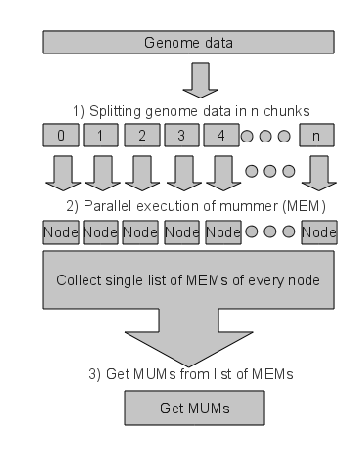
\epsfig{file=algorithm.eps,width=4.5cm,height=4cm} 
\end{center} 
\caption{Data-level parallelism technique for whole genome alignment.} 
\label{algorithm} 
\end{figure} 
To verify that our approach, Xipe Totec, can align a whole genome a set of tests were analyzed. These tests were carried out in a cluster with the following features:
\begin{itemize}
\item Hardware: 
\begin{itemize}
\item Processor Dual-Core Intel(R) Xeon(R) CPU 5160 @ 3.00GHz 4MB L2 (2x2)
\item Number of processors: 2
\item RAM: 12 GB Fully Buffered DIMM 667 MHz
\end{itemize}
\item  Software:
\begin{itemize}
\item Linux Kernel 2.6.16.46-0.12-smp x86\_64 GNU/Linux
\item gcc 4.3.2
\item MUMmer 3.22
\item Perl 5.8.8
\end{itemize}
\end{itemize}
Each genome alignment was executed following these phases:
\begin{itemize}
\item Split genome data:
\begin{itemize}
\item Genome size: 115,86 Mbp\footnote{Two nitrogenous bases paired together in double-stranded DNA by weak bonds; specific pairing of these bases (adenine with thymine and guanine with cytosine) facilitates accurate DNA replication; when quantified (e.g., 8 bp), refers to the physical length of a sequence of nucleotides \cite{ncbi}}.
\item Division of genome in 2, 4, 8, 16 chunks.
\item An overlapping size of 5000bp.
%  \begin{enumerate}
%    \item 100 Kbp
%    \item 250 Kbp
%    \item 500 Kbp
%    \item 2500 Kbp
%    \item 5000 Kbp
%  \end{enumerate}
\end{itemize}
\item Test for several size of MEMs:
  \begin{enumerate}
    \item 20 bp
    \item 50 bp
    \item 100 bp
    \item 500 bp
    \item 1000 bp
  \end{enumerate} 
\end{itemize}
Then each way of parallelization is executed:
\begin{itemize}
\item Align the query genome by splitting it against a global whole reference genome, see Figure \ref{splitqry}.
\begin{figure}[htb] 
  \begin{center}
    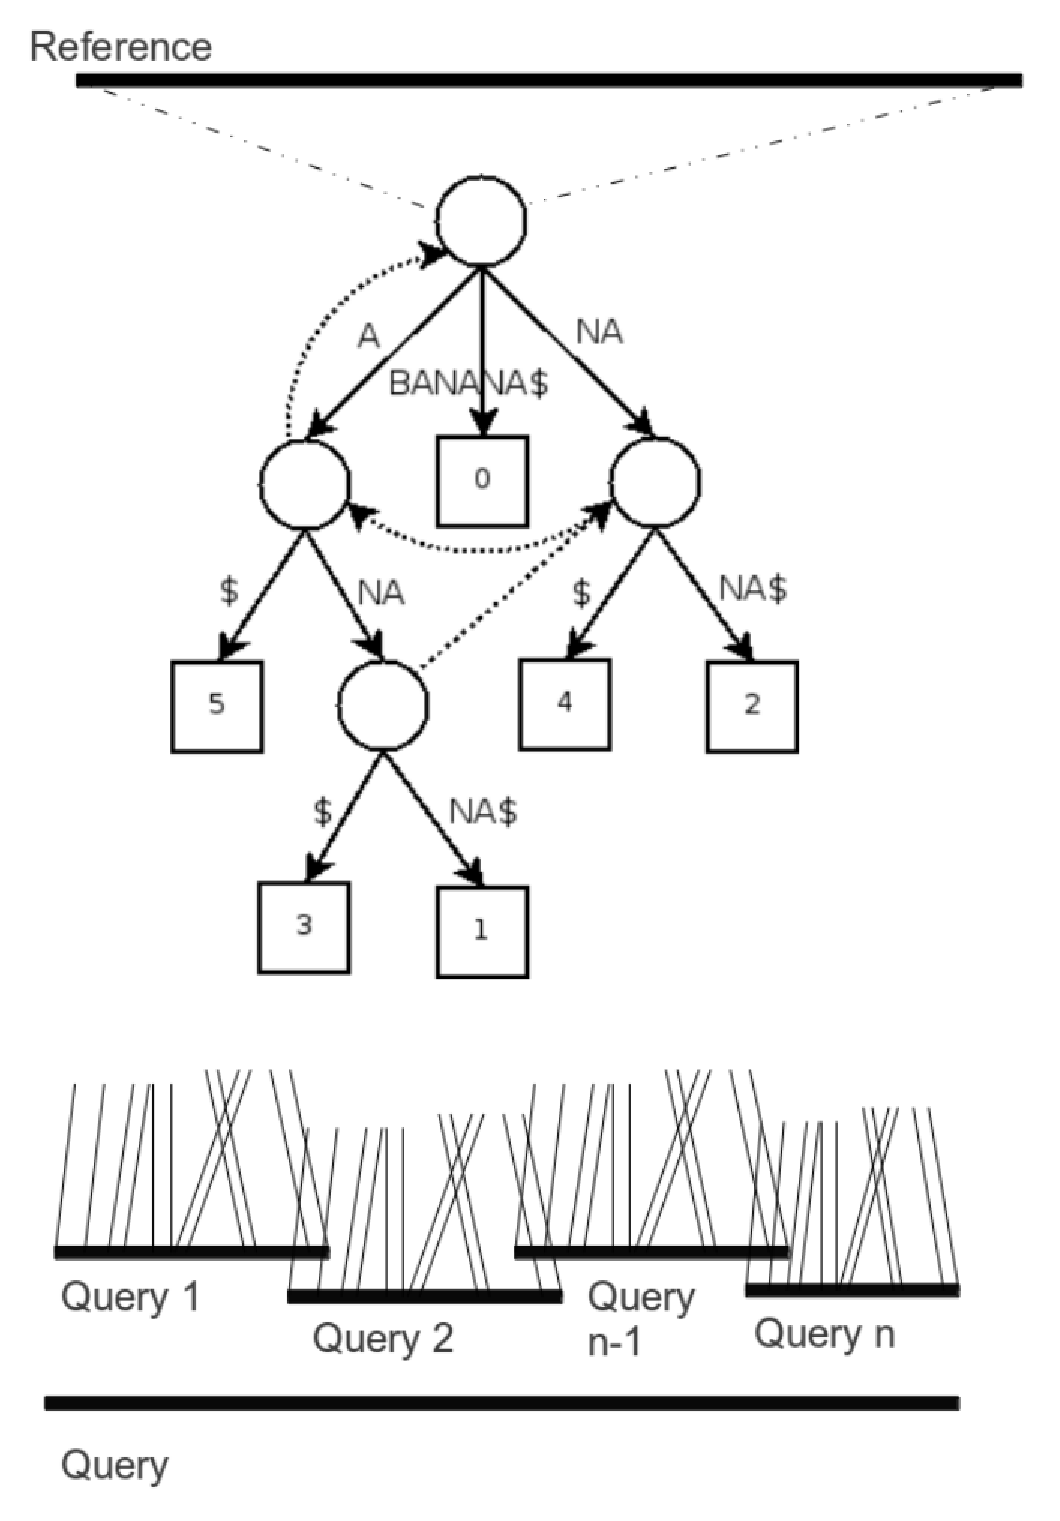
\epsfig{file=split_qry.eps,width=5cm,height=4cm}
  \end{center}
 \caption{Split query genome.}
 \label{splitqry}
\end{figure}
\item Align the whole query genome against every chunk of reference genome, see Figure \ref{splitref}.
\begin{figure}[htb]
  \begin{center}
    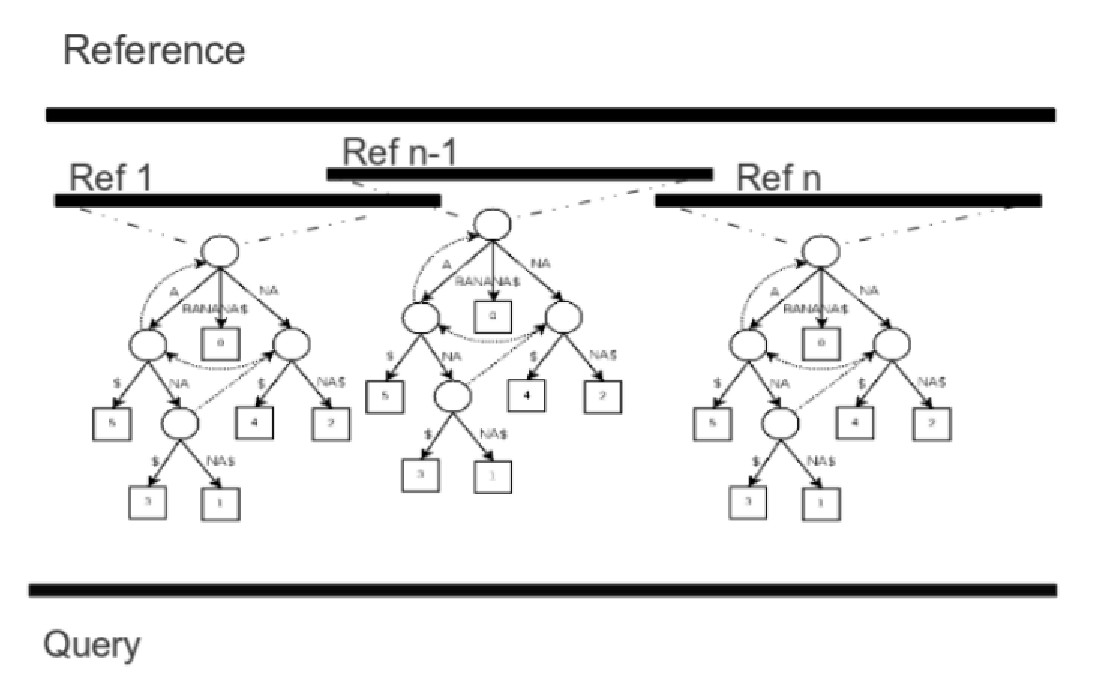
\epsfig{file=split_ref.eps,width=7.5cm}
  \end{center}
 \caption{Split reference genome.}
 \label{splitref}
\end{figure}
\end{itemize}
Our was with the human chromosome 13 as reference genome and the chimpanzee chromosome 13 as query genome. The correct size of each genome is:
\begin{itemize}
  \item Human chromosome 13: 95.78 Mbp
  \item Chimpanzee chromosome 13: 115,86 Mbp
\end{itemize}
The first parameter to measure was the construction of suffix tree. In Figure \ref{hspan_st_r} is shown how, a division of reference genome improves the building time of suffix tree, up to 27 times when the reference is divided in 16 chunks. Though a quick build of suffix tree is achieved when the reference is split the but this improvement is not possible when the query genome is split, in Figure \ref{hspan_st_q} is shown the building time for suffix tree which remains constant.
\begin{figure}[htb] 
\centering
\subfloat[][Construction of ST split Human Chr13 reference.]
{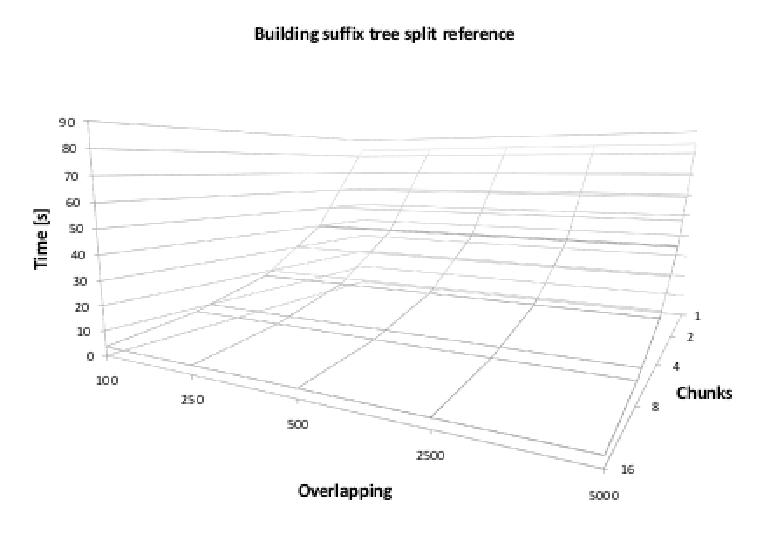
\epsfig{file=hspan_st_r.eps,width=3.4cm} \label{hspan_st_r}}
\hspace{0.1cm}
\subfloat[][Construction of ST split Chimpanzee Chr13 query.]
{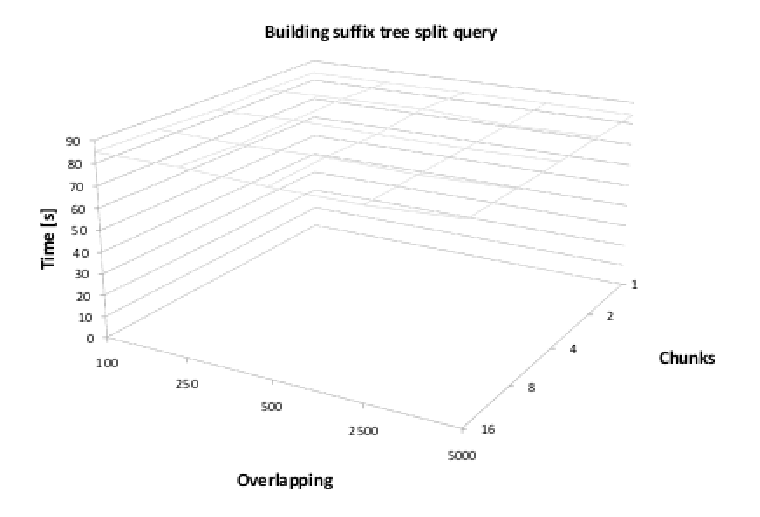
\epsfig{file=hspan_st_q.eps,width=3.4cm} \label{hspan_st_q}}
\end{figure}
The second parameter to test was the computation time to find the MEMs. As it was explained in the previous chapter we follow a brute-force approach to get the same list of MUMs when our technique is used. In other words, it might be possible that for some genome sizes our approach can be worse than the sequential version.\\
In the Figure \ref{hspan_find_r_5000} is shown the several configurations tested when the reference genome is split. \\
It is important to point out that this test shows that for some configurations our approach does not work at all: when the Match length is very short, like 20 bp. The answer to this problem is that when a small match is searched in a big genome the number of matches can become exponentially. This undesirable feature can be seen in Figure \ref{hspan_drop} and Figure \ref{hspan_mums} which shows the high number of hits when a short match is searched.\\
\begin{figure}[htb] 
\centering
\subfloat[][Finding MEMs split Human Chr13, Overlap=5000bp.]
{\epsfig{file=hspan_find_r_5000.eps,width=3.2cm} \label{hspan_find_r_5000}}
\hspace{0.1cm}
\subfloat[][Finding MEMs split Chimpanzee Chr13, Overlap=5000bp.]
{\epsfig{file=hspan_find_q_5000.eps,width=3.2cm} \label{hspan_find_q_5000}}
\end{figure}
On the other hand when the query genome is split the reduction of time to find MEMs is only of the magnitude of 20\%.\\
Memory usage is a big issue when a genome goes from a few Mbp to hundreds of Mbp, our reference genome is almost 100Mbp and the requirement for memory can be seen in Figure \ref{hspan_ram}. For a genome of 95Mbp, the algorithm requires more than 1.6GB, from our experiments we can show that if we divide genome reference in 16 chunks, memory requirement reduces to only 12.5\% of the sequential version use of memory.\\
\begin{figure}[htb] 
\begin{center}
      \epsfig{file=hspan_ram.eps,width=7.5cm}
    \caption{Use of memory when aligning Human Chr13 vs. Chimpanzee Chr13.}
    \label{hspan_ram}
  \end{center}
\end{figure}
The most important step in our test was to verify that our parallelization can get the same alignment (same list of MUMs from the sequential version), in Figures \ref{hspan_mums}, \ref{hspan_mums_20}, \ref{hspan_mums_50}, \ref{hspan_mums_100}, \ref{hspan_mums_500} and \ref{hspan_mums_1000} reader can watch the list of MUMs which should be the same when we apply our parallelization technique. In order to know if our approach does the job we filter those matches which are MUMs. To understand this point, the Figure \ref{hspan_drop} shows the number of matches discarded.
\begin{figure}[htb] 
\centering
\subfloat[][List of MUMS for several sizes of MUM when aligning Human Chr13 vs. Chimpanzee Chr13.]
{\epsfig{file=hspan_mums.eps,width=3.2cm} \label{hspan_mums}}
\hspace{0.1cm}
\subfloat[][Percentage of dropped MEMs in order to get the same list of MUMs for the sequential version of MUMmer, when aligning Human Chr13 vs. Chimpanzee Chr13.]
{\epsfig{file=hspan_drop.eps,width=3.2cm} \label{hspan_drop}}
\end{figure}
\begin{figure}[htb] 
\centering
\subfloat[][Frequency of MUMs, length of 20bp, found when aligning Human Chr13 vs. Chimpanzee Chr13.]
{\epsfig{file=hspan_mums_20.eps,width=3.2cm} \label{hspan_mums_20}}
\hspace{0.1cm}
\subfloat[][Frequency of MUMs, length of 50bp, found when aligning Human Chr13 vs. Chimpanzee Chr13.]
{\epsfig{file=hspan_mums_50.eps,width=3.2cm} \label{hspan_mums_50}}
\end{figure}
\begin{figure}[htb] 
\centering
\subfloat[][Frequency of MUMs, length of 100bp, found when aligning Human Chr13 vs. Chimpanzee Chr13.]
{\epsfig{file=hspan_mums_100.eps,width=3.2cm} \label{hspan_mums_100}}
\hspace{0.1cm}
\centering
\subfloat[][Frequency of MUMs, length of 500bp, found when aligning Human Chr13 vs. Chimpanzee Chr13.]
{\epsfig{file=hspan_mums_500.eps,width=3.2cm} \label{hspan_mums_500}}
\end{figure}
\begin{figure}[htb] 
\centering
\subfloat[][Frequency of MUMs, length of 1000bp, found when aligning Human Chr13 vs. Chimpanzee Chr13.]
{\epsfig{file=hspan_mums_1000.eps,width=3.2cm} \label{hspan_mums_1000}}
\end{figure}
\subsection*{Drawbacks}
Our novel approach has some limitations which are listed below:
\begin{itemize}
  \item It can work well with genome data of size less than 100Mbp.
  \item The use of a short match length can heavily impact in performance of our approach.
  \item This technique does not provide any feature of checkpoint.
  \item Our approach does not take advantage of any parallel programming language (OpenMP, OpenMPI, etc.).
\end{itemize}
These drawbacks are some opportunities to work with in the near future.\\
In addition, there are more issues related to computational tasks like a fair usage of available resources to do whole genome alignment. Among the desirable attributes any whole genome alignment algorithm should have are:
\begin{itemize}
\item Time: in order to be able to process whole genomes.
\item Space: a clever use of data structures to not run out of memory. 
\end{itemize}
Both of these attributes were enhanced in MUMmer to provide a first approach to whole genome alignment in HPC clusters.

%%%%%%%%%%%%%%%%%%%%%%
\section*{Conclusions}
We have set in place a parallelization of whole genome alignment, Xipet Totec, and used MUMmer to evaluate the alignment of two genomes. We have found that a data level parallelism allows an approximation of a correct alignment.\\
We view this work as a starting point toward the goal of completely automating alignment parallelization. In addition to split data genome, we will also need to automatically choose seeding strategies and thresholds. \\
This work has made some progress, especially in improved pairwise alignment with a heuristic basis, which has shown the efficiency to handle memory management and the parallel distribution of genome data in order to get a quicker whole genome alignment. Additionally, a better heuristic should be used to allow the full use of clusters and multicore architectures. This new heuristic may improve the finding of matches so that every process can handle its chunk and it could notice if a match is unique or not by checking the other chunks. In this way a new concept of distributed MUM is defined:
\begin{center}
\begin{mydef}
Distributed Maximal Unique Match(DMUM) substring is a common substring of the two genomes that is longer than a specific minimum length d such that it is maximal, that is, it cannot be extended on either end without incurring a mismatch and it is unique in any of the chunks of the genome.
\end{mydef}
\end{center}
DMUM works by checking first if it is a MUM locally and then asking to the other chunks if this MUM is a real MUM in the whole genome. The DMUM has the advantage of having less intermediate data (MEMs) but with an overhead of communications between each chunk and the computation time to check if the match is unique or not.\\
Our technique is a startup to explore the multiple faces of bioinformatics to do a better use of the available computer resources. This work shows that a novel parallelization and the knowledge of genome data can improve the run time and memory.\\
Several configurations were tested and some drawbacks were found. The main restriction to implement this technique  is the  limited memory resource in our environment test.
  
%%%%%%%%%%%%%%%%%%
\section*{Methods}
The sequential version of the MUMmer's algorithm trades extra computation for memory and high computation time when executed in a single machine. \\
Previously the algorithm for sequence alignment was described in detail. Now our own proposal of a parallelization of WGA with MUMmer is explained, Xipe Totec. There are two resources to improve in this algorithm:
\begin{itemize}
\item Memory usage.
\item Running time.
\end{itemize}
To improve the performance of the algorithm a data-level parallelism technique is deployed in advance to genome alignment.\\
Our technique is divided in three phases following:
\begin{enumerate}
\item Splitting genome data according to the number of available cores.
\item Parallel execution of as many instances of mummer as available cores.
\item Get the list of MUMs from the whole set of MEMs\footnote{Maximal Exact Match} found in the previous phase.
\end{enumerate}
The division of genome data was used using the paradigm of data-level parallelism which consists of a generation of chunks of a sequence with a fixed size and a fixed overlap. One issue arises when a genome is splitted because of the heuristic used in the algorithm is affected. So that, a longer sequence is more likely to have a better finding of MUMs while a smaller one can produce MUMs which are not effective MUMS.\\
Another consideration was the genome structure, because a genome is build from a finite alphabet $\Sigma=\{a,g,c,t,n\}$ but according to the MUMmer's algorithm each alignment is made using only the nucleotide base pairs, this means that letter "n" in a biological way can mean anything: (a,g,c,t). A complex structure of a genome can have a huge impact of our data level parallelism.\\
To get a MUM, it requires an important feature its uniqueness. 
Uniqueness can only be found when a whole genome is checked.
In other words, after finding MUMs within a chunk it is not possible to determine if the MUM found is or not a "unique" MUM, globally in the genome,  because these MUMs are unique only in the chunk that has been read, the rest of the genome it is not known.\\
One solution to solve this problem is to drop the MUMmer's heuristic in order to be able to find the correct MUMs when we apply our data-level parallelism. The new approach is to find a Maximal Exact Match (MEM), a MEM allows to drop the uniqueness of a match but with a high computational cost: a brute-force approach.\\
Nevertheless, the major problem with the use of MEM is that the number of occurrences increases exponentially when \emph{shorter MEM} are used. Moreover, the high ratio of MEMs requires to save them in some place, memory or disk, that means a heavy use of resources in both CPU and Memory. This drawback is the main disadvantage because the hits of MEMs are increasing with the size of the genome. A new phase has to be designed to reduce the use of resources when a short MEM is searched.
\subsection*{Implementation} 
\label{implementation}
This section explains in detail how our proposal is implemented and the modifications in order to be executed in MUMmer. The following diagram, see Figure \ref{xipe-totec}, shows the add-ons of our approach, one is executed before MUMmer and the another after MUMmer.
\begin{figure}[htb]  
 \begin{center} 
    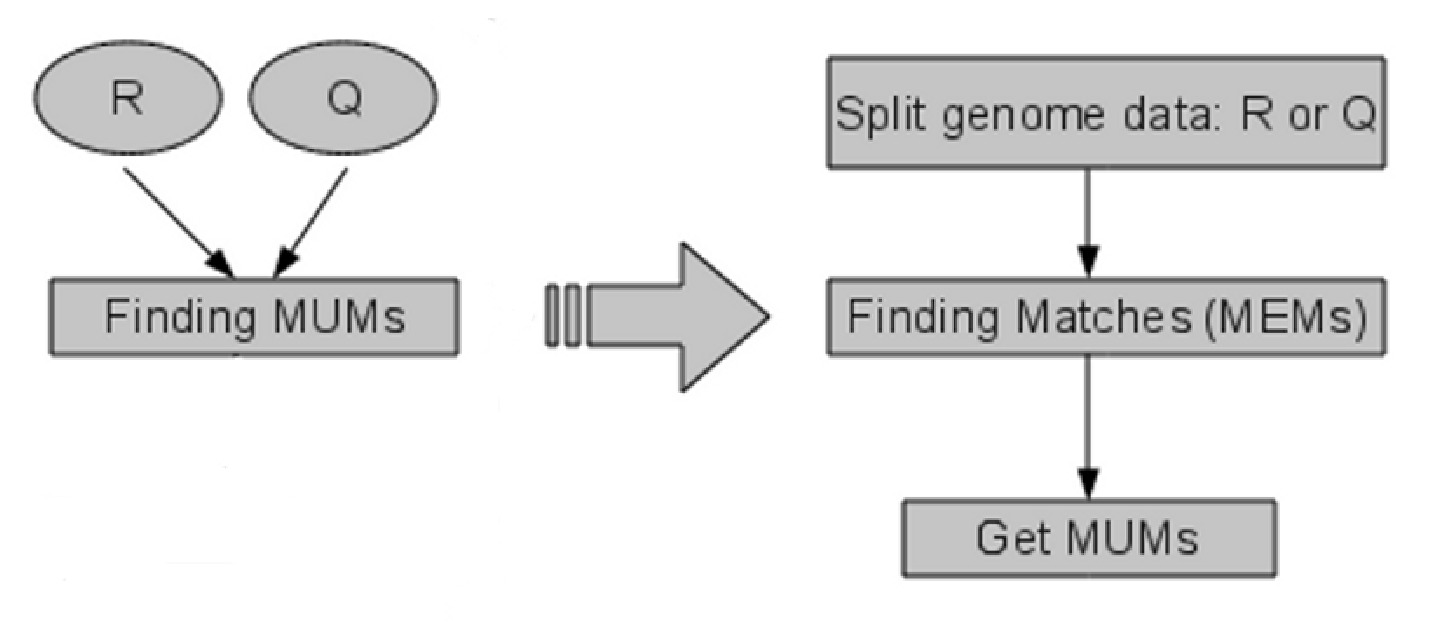
\epsfig{file=xipe-totec1.eps,width=7.5cm} 
 \end{center}
 \caption{Xipe Totec: proposal for parallelization of whole genome alignment} 
 \label{xipe-totec} 
\end{figure}
The following sections explain how the split of genome data, search of MEMs and get MUMs are carried out in our proposal.
\subsubsection*{Split genome data} 
As it was previously explained, the approach is to use a fixed size division of genome data in as many chunks as  many available cores. Xipe Totec needs to know how many cores will be used in order to divide the genome data.\\
One key aspect of Xipe Totec is the way to split a genome. To align a genome requires a reference genome so that, there are two ways of using Xipe Totec:
\begin{itemize}
\item Splitting reference genome.
\item Splitting query genome.
\end{itemize}
Both of them can reduce the computation time or memory usage.\\
To split genome data a perl script was coded to do this task, the script requires the following arguments:
\begin{itemize}
\item Genome data to be splitted.
\item Number of chunks.
\item Overlap size.
\item Location to save the genome data.
\end{itemize}
\subsubsection*{Finding MEMs}
This phase requires the mummer program, one of the several small programs in the MUMmer suite. mummer has several options.
In order to get a correct alignment, our proposal requires to compute MEMs instead of MUMs, so that mummer is executed with:
\begin{itemize}
  \item -n: to match only nucleotides.
  \item -maxmatch: option to get MEMs.
  \item -l \emph{length}: to find MEMs of a some minimum length.
\end{itemize}
List of MEMs is saved to a file which has the following format:
\begin{verbatim}
>Information about the sequence
Position_in_R Position_in_Q Length_of_MEM
\end{verbatim}
This list has to be joined with the output of every chunk computed and then the whole list is  manipulated in the following phase, \ref{getting}.
\subsection{Getting MUMs}
\label{getting}
This is the most important phase in our approach because it outputs the final list of MUMs those that are the same to the serial execution of mummer.\\
This phase needs the list of MEMs to process them and find those matches that are unique. The following diagram shows the basic idea behind this phase, see Figure \ref{xt}.
\begin{figure}[htb]  
 \begin{center} 
   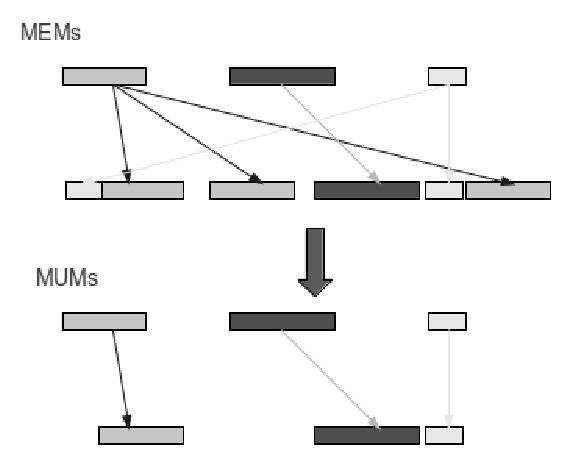
\epsfig{file=xt.eps,width=5cm, height=2cm} 
 \end{center} 
 \caption{Xipe Totec: Finding the real MUMs} 
   \label{xt} 
\end{figure}
To get the MUMs we filter those MEMs that are unique in the list and order them using a modified version of LIS\footnote{Longest Increasing Subsequence} algorithm.
The algorithm is shown below:
\begin{algorithmic}
\STATE{Input: List of MEMs: Position in R, position in Q, length of MEM}
\STATE{Sort MEMs by increasing position and decreasing length in R}
\FOR{$i:=0$ to $n$ in Total\_MEMs}
\IF{MEM[$i$] is not unique}
\STATE{Sort this subset by increasing position in Q and pick up the first MEM and drop the rest}
\ELSE {}
\STATE{MEM[$i$] is a MUM}
\ENDIF
\ENDFOR
\STATE{Sort MEMs by increasing position and decreasing length in Q}
\FOR{$i:=0$ to $n$ in Total\_MEMs}
\IF{MEM[$i$] is not unique}
\STATE{Sort this subset by increasing position in R and pick up the first MEM and drop the rest}
\ELSE {}
\STATE{MEM[$i$] is a MUM}
\ENDIF
\ENDFOR
\end{algorithmic}
The output of this algorithm gives the MUMs.
%%%%%%%%%%%%%%%%%%%%%%%%%%%%%%%%
\section*{Authors contributions}
 JCGV carried out the design and evaluation of the technique described and drafted the manuscript.\\
 AE helped to draft the manuscript.

%%%%%%%%%%%%%%%%%%%%%%%%%%%
\section*{Acknowledgements}
  \ifthenelse{\boolean{publ}}{\small}{}
This work was supported by grant from Ejecuci\'on eficiente de aplicaciones multidisciplinares: nuevos desaf\'ios en la 
era multi/many core, with reference TIN2011-28689-C02-01.

 
%%%%%%%%%%%%%%%%%%%%%%%%%%%%%%%%%%%%%%%%%%%%%%%%%%%%%%%%%%%%%
%%                  The Bibliography                       %%
%%                                                         %%              
%%  Bmc_article.bst  will be used to                       %%
%%  create a .BBL file for submission, which includes      %%
%%  XML structured for BMC.                                %%
%%                                                         %%
%%                                                         %%
%%  Note that the displayed Bibliography will not          %% 
%%  necessarily be rendered by Latex exactly as specified  %%
%%  in the online Instructions for Authors.                %% 
%%                                                         %%
%%%%%%%%%%%%%%%%%%%%%%%%%%%%%%%%%%%%%%%%%%%%%%%%%%%%%%%%%%%%%


{\ifthenelse{\boolean{publ}}{\footnotesize}{\small}
 \bibliographystyle{bmc_article}  % Style BST file
  \bibliography{wga_APBC2012} }     % Bibliography file (usually '*.bib' ) 

%%%%%%%%%%%

\ifthenelse{\boolean{publ}}{\end{multicols}}{}

%%%%%%%%%%%%%%%%%%%%%%%%%%%%%%%%%%%
%%                               %%
%% Figures                       %%
%%                               %%
%% NB: this is for captions and  %%
%% Titles. All graphics must be  %%
%% submitted separately and NOT  %%
%% included in the Tex document  %%
%%                               %%
%%%%%%%%%%%%%%%%%%%%%%%%%%%%%%%%%%%

%%
%% Do not use \listoffigures as most will included as separate files

\section*{Figures}
  \subsection*{Figure 1 - schema.eps}
    Operations in whole genome alignment.
  \subsection*{Figure 2 - Sample figure title}
      Figure legend text.



%%%%%%%%%%%%%%%%%%%%%%%%%%%%%%%%%%%
%%                               %%
%% Tables                        %%
%%                               %%
%%%%%%%%%%%%%%%%%%%%%%%%%%%%%%%%%%%

%% Use of \listoftables is discouraged.
%%
\end{document}







